\documentclass[11pt]{article}

\usepackage{graphicx}

\marginparwidth 0.5in 
\oddsidemargin 0.25in 
\evensidemargin 0.25in 
\marginparsep 0.25in
\topmargin 0.0in 
\textwidth 6in \textheight 8.5in

\title{sQuire: A Web Based Collaborative Editor\\Homework 2 Individual Work\\Group 4}
\author{Rick Boss (boss2849)}

\begin{document}
\maketitle

\newpage
\tableofcontents
\newpage

\section{Use Case Diagram}
\subsection{Project User Management (boss2849)}
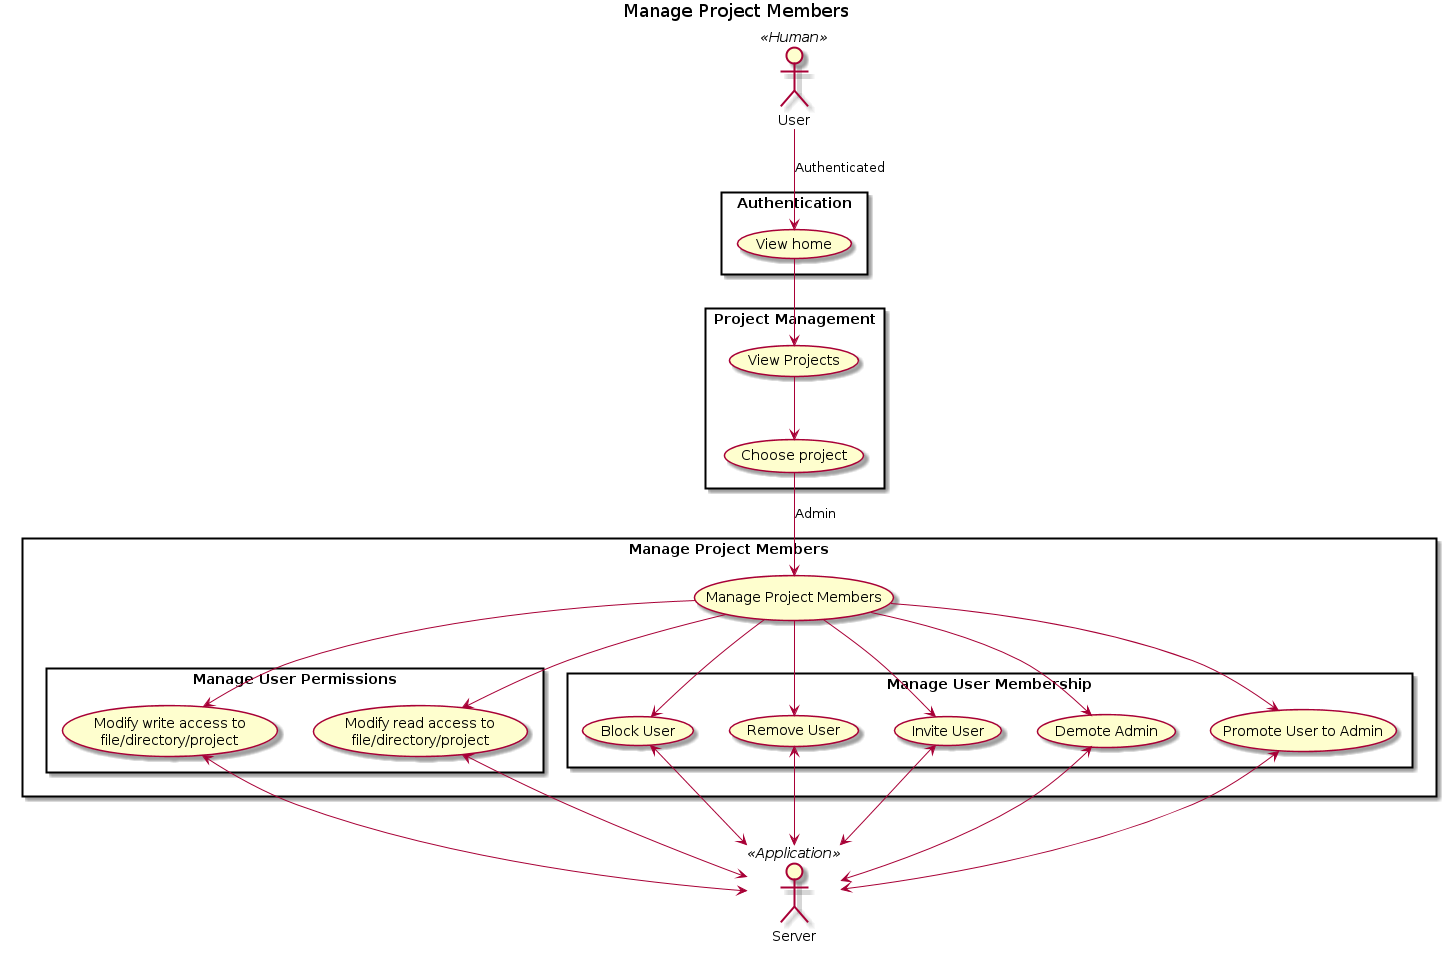
\includegraphics[width=1\textwidth]{../uml-diagram/user-management}
Use case diagram depicting Project User Management features for sQuire.

\section{Use Case Descriptions}
\subsection{Project User Management (boss2849)}
\subsubsection{Modify read/write access (boss2849)}
\begin{tabular}{ p{2cm} p{12cm} }
 \hline
 \\
 \textit{Actors:} & User \\ 
 \\
 \textit{Goals:} & Modify a user\'s permissions. \\
 \\
 \textit{Pre-conditions:} & User is signed in and holds Admin rights for the currently selected Project\\
 \\
 \textit{Summary:} & User modifies another User\'s read/write permissions to portions of the project. \\
 \\
 \textit{Related use cases:} & None. \\ 
 \\
 \textit{Steps:} & \begin{enumerate}
  \item User clicks Permissions Management
  \item System displays permissions management window
  \item User selects a file, multiple files, directory or entirety of project and grants/revokes read/write access
  \item System modifes the target User\'s permissions and notifies them.
 \end{enumerate} \\
 \\
 \textit{Alternatives:} & 3. User selects cancel, System discards changes. \\
 \\
 \textit{Post-conditions:} & None. \\
 \\
\hline
\end{tabular}

\subsubsection{Remove User  (boss2849)}
\begin{tabular}{ p{2cm} p{12cm} }
 \hline
 \\
 \textit{Actors:} & User \\ 
 \\
 \textit{Goals:} & Remove a user from project. \\
 \\
 \textit{Pre-conditions:} & User is signed in, in project with Admin rights, and is on User Management page\\
 \\
 \textit{Summary:} & User removes a selected user from the Project \\ 
 \\
 \textit{Related use cases:} & Invite User, Modify Read/Write Access \\ 
 \\
 \textit{Steps:} & \begin{enumerate}
  \item User clicks Remove User button.
  \item System displays list of active users for project.
  \item User selects one or more other users from the list and presses Remove.
  \item System prompts User for verification.
  \item User presses Confirm.
  \item System removes the selected users from the project.
  \item System revokes read and write access from the selected users.
  \item System notifies selected users that they have been removed from the project.
 \end{enumerate} \\
 \\
 \textit{Alternatives:} & User presses Cancel in steps 3 or 5, System returns user to User Management page \\
 \\
 \textit{Post-conditions:} & None. \\
 \\
\hline
\end{tabular}

\subsubsection{Invite User to Project  (boss2849)}
\begin{tabular}{ p{2cm} p{12cm} }
 \hline
 \\
 \textit{Actors:} & User \\ 
 \\
 \textit{Goals:} & Invite user(s) to project \\
 \\
 \textit{Pre-conditions:} & User is signed in, in project with Admin rights, and is on User Management page \\
 \\
 \textit{Summary:} & User invites user(s) to the current project. \\ 
 \\
 \textit{Related use cases:} & Remove User, Join Project \\ 
 \\
 \textit{Steps:} & \begin{enumerate}
  \item User clicks Invite Users button
  \item System prompts user to enter username(s)/email(s)
  \item User enters username(s)/email(s) of the user(s) to invite and presses Ok.
  \item System looks up the specified user(s) and notifies them of invitation to the Project
 \end{enumerate} \\
 \\
 \textit{Alternatives:} & \begin{enumerate}
  \item User presses cancel in step 3, System returns User to User Management page
  \item In step 4, username(s)/email(s) don\'t match any users, System notifies User of failed invitiations.
 \end{enumerate} 
 \\
 \textit{Post-conditions:} & None. \\
 \\
\hline
\end{tabular}

\subsubsection{Promote User to Admin  (boss2849)}
\begin{tabular}{ p{2cm} p{12cm} }
 \hline
 \\
 \textit{Actors:} & User \\ 
 \\
 \textit{Goals:} & Promote a specified User to Admin \\
 \\
 \textit{Pre-conditions:} & User is signed in, in project with Admin rights, and is on User Management page \\
 \\
 \textit{Summary:} & User selects another User to be given Admin rights for the project. \\ 
 \\
 \textit{Related use cases:} & Demote Admin \\ 
 \\
 \textit{Steps:} & \begin{enumerate}
  \item User selects Promote to Admin.
  \item System displays a list of non-Admin active users.
  \item User selects user(s) and presses Submit.
  \item System prompts user for confirmation.
  \item User selects Confirm.
  \item System grants Admin permissions to the selected user(s).
 \end{enumerate} \\
 \\
 \textit{Alternatives:} & User presses cancel in steps 3 or 5, no action taken. \\
 \\
 \textit{Post-conditions:} & None. \\
 \\
\hline
\end{tabular}

\subsubsection{Demote Admin  (boss2849)}
\begin{tabular}{ p{2cm} p{12cm} }
 \hline
 \\
 \textit{Actors:} & User \\ 
 \\
 \textit{Goals:} & Demote Admin to user \\
 \\
 \textit{Pre-conditions:} & User is signed in, in project with Admin rights, and is on User Management page \\
 \\
 \textit{Summary:} & User demotes selected Admins to normal Users for the project. \\ 
 \\
 \textit{Related use cases:} & Promote User to Admin \\ 
 \\
 \textit{Steps:} & \begin{enumerate}
  \item User selects Demote Admin
  \item System displays list of Admins
  \item User selects Admin(s) to demote and presses Submit.
  \item System prompts User for confirmation.
  \item User presses Confirm.
  \item System revokes Admin rights from selected User(s)
 \end{enumerate} \\
 \\
 \textit{Alternatives:} & \begin{enumerate}
  \item User presses cancel in steps 3 or 5, no action taken
  \item User attempts to demote Admin that is the Owner of the project, System rejects request and notifies User.
 \end{enumerate}
 \\
 \textit{Post-conditions:} & None. \\
 \\
\hline
\end{tabular}

\subsubsection{Block User (boss2849)}
\begin{tabular}{ p{2cm} p{12cm} }
 \hline
 \\
 \textit{Actors:} & User \\ 
 \\
 \textit{Goals:} & Block a user from the project \\
 \\
 \textit{Pre-conditions:} & User is signed in, in project with Admin rights, and is on User Management page \\
 \\
 \textit{Summary:} & User blocks a user from the project, making them unable to view the project. \\ 
 \\
 \textit{Related use cases:} & Demote Admin \\ 
 \\
 \textit{Steps:} & \begin{enumerate}
  \item User clicks Block User.
  \item System displays a list of active users.
  \item User selects other user(s) to block and presses Submit.
  \item System prompts User for confirmation.
  \item User presses Confirm.
  \item System blocks selected user(s) from the project, revoking read/write access, and revoking Admin status as necessary.
 \end{enumerate} \\
 \\
 \textit{Alternatives:} & User presses cancel in steps 3 or 5.
 \\
 \textit{Post-conditions:} & None. \\
 \\
\hline
\end{tabular}

\end{document}
